% !TeX TXS-program:compile = txs:///pdflatex/[--shell-escape]
%
% acm templates v1.57 (sigconf template)
%
%\documentclass[sigconf, screen, review, anonymous, natbib=false]{acmart}
\documentclass[sigconf, screen, natbib=false, dvipsnames, table]{acmart}
\settopmatter{printacmref=true}
% mandatory for CCS'19
\usepackage{balance}
% for creating a balanced last page (usually last page with references)

% defining the \BibTeX command - from Oren Patashnik's original BibTeX documentation.
\def\BibTeX{{\rm B\kern-.05em{\sc i\kern-.025em b}\kern-.08emT\kern-.1667em\lower.7ex\hbox{E}\kern-.125emX}}

% Rights management information. 
% This information is sent to you when you complete the rights form.
% These commands have SAMPLE values in them; it is your responsibility as an author to replace
% the commands and values with those provided to you when you complete the rights form.
%
% These commands are for a PROCEEDINGS abstract or paper.

\copyrightyear{2019} 
\acmYear{2019} 
\setcopyright{acmcopyright}
\acmConference[CCS '19]{2019 ACM SIGSAC Conference on Computer and Communications Security}{November 11--15, 2019}{London, United Kingdom}
\acmBooktitle{2019 ACM SIGSAC Conference on Computer and Communications Security (CCS '19), November 11--15, 2019, London, United Kingdom}
\acmPrice{15.00}
\acmDOI{10.1145/3319535.3339818}
\acmISBN{978-1-4503-6747-9/19/11}

%
% These commands are for a JOURNAL article.
%\setcopyright{acmcopyright}
%\acmJournal{TOG}
%\acmYear{2018}\acmVolume{37}\acmNumber{4}\acmArticle{111}\acmMonth{8}
%\acmDOI{10.1145/1122445.1122456}

%
% Submission ID. 
% Use this when submitting an article to a sponsored event. You'll receive a unique submission ID from the organizers
% of the event, and this ID should be used as the parameter to this command.
%\acmSubmissionID{123-A56-BU3}

%
% The majority of ACM publications use numbered citations and references. If you are preparing content for an event
% sponsored by ACM SIGGRAPH, you must use the "author year" style of citations and references. Uncommenting
% the next command will enable that style.
%\citestyle{acmauthoryear}


 \makeatletter
 % \renewcommand{\section}{\abovedisplayskip 10\p@ \@plus3\p@ \@minus1\p@%
 %                       \belowdisplayskip 5\p@ \@plus3\p@ \@minus1\p@%
 %                       \abovedisplayshortskip 0pt \@plus2\p@%
 %                       \belowdisplayshortskip 0pt \@plus2\p@ \@minus0\p@%
 %                       \@startsection{section}{1}{\z@}%
 %                        {-17\p@ \@plus -4\p@ \@minus -4\p@}%
 %                        {6\p@ \@plus 4\p@ \@minus 4\p@}%
 %                        {\normalfont\large\bfseries\boldmath
 %                         \rightskip=\z@ \@plus 8em\pretolerance=10000 }}
 \renewcommand{\subsection}{\@startsection{subsection}{2}{\z@}%
                        {-8\p@ \@plus -4\p@ \@minus -4\p@}%
                        {5\p@ \@plus 2\p@ \@minus 2\p@}%
                        {\normalfont\Large\bfseries\boldmath
                         \rightskip=\z@ \@plus 3em\pretolerance=10000 }}
  \renewcommand{\subsubsection}{\@startsection{subsubsection}{3}{\z@}%
                        {-6\p@ \@plus -4\p@ \@minus -4\p@}%
                        {1\p@ \@plus 1\p@ \@minus 0\p@}%
                        {\normalfont\normalsize\bfseries\boldmath}}
% \renewcommand{\paragraph}{\@startsection{paragraph}{4}{\z@}%
%                       {-8\p@ \@plus -4\p@ \@minus -4\p@}%
%                       {-2\p@ \@plus -0.22em \@minus -0.1em}%
%                       {\normalfont\normalsize\bfseries}}
 \makeatother



% *** GRAPHICS RELATED PACKAGES ***
\usepackage{graphicx}
\usepackage{comment}
\usepackage{amsmath,amssymb,amsfonts}
\usepackage{listings}
% declare the path(s) where your graphic files are
\graphicspath{{../figures/}}
% and their extensions so you won't have to specify these with
% every instance of \includegraphics
\DeclareGraphicsExtensions{.pdf,.jpeg,.png}

%\usepackage[outputdir=/Volumes/ramdisk/]{minted}
\usepackage{minted}
% *** MATH PACKAGES ***
\usepackage{amsmath}



% *** SPECIALIZED LIST PACKAGES ***
\usepackage{algorithmic}




% *** ALIGNMENT PACKAGES ***
\usepackage{array}

\usepackage{url}

\usepackage[utf8]{inputenc}
\usepackage[american]{babel}
\usepackage[backend=biber,style=ACM-Reference-Format]{biblatex}
\addbibresource{../library.bib} 
\addbibresource{../cryptobib/abbrev2.bib}
\addbibresource{../cryptobib/crypto_crossref.bib}

% Used for Theorems and Definitions
\usepackage{amsthm}
\newtheorem{definition}{Definition}
\newtheorem{theorem}{Theorem}
\newtheorem{lemma}{Lemma}
\theoremstyle{definition}
\newtheorem{remark}{Remark}

\usepackage{xcolor} 
\usepackage{xspace}
\usepackage{xstring} % required by IfEqCase

\usepackage{booktabs} % better tables

% ishaq: adding our macros

% the following commands require xcolor and xpace packages
\newcommand{\vassilis}[1]{{\color{blue} {\sc Vassilis:} \it #1}\xspace}
\newcommand{\vvassilis}[1]{{\color{blue} \footnote{\vassilis{#1}}}}
%\renewcommand{\vvassilis}[1]{\vassilis{#1}}

\newcommand{\ana}[1]{{\color{red} {\sc Ana:} \it #1}\xspace}
\newcommand{\aana}[1]{{\color{red} \footnote{\ana{#1}}}}
\newcommand{\ishaq}[1]{{\color{teal} {\sc Ishaq:} \it #1}\xspace}
\newcommand{\iishaq}[1]{{\color{teal} \footnote{\ishaq{#1}}}}
\newcommand{\ben}[1]{{\color{orange} {\sc Ben:} \it #1}\xspace}
\newcommand{\bben}[1]{{\color{orange} \footnote{\ben{#1}}}}
\newcommand{\benjamin}[1]{{\color{green} {\sc Benjamin:} \it #1}\xspace}

\newcommand{\revised}[1]{#1}
\newcommand{\brevised}[1]{{\color{blue} #1}}

\newcommand{\rrefer}[2]{%
    \IfEqCase{#1}{%
        {proceedings}{\revised{See full version for details.}}%
        {full}{\revised{See appendix~\ref{#2} for details.}}%
        % you can add more cases here as desired
    }[\PackageError{rrefer}{Undefined option for arg1 #1}]%
}
\newcommand{\refer}[1]{\rreferx{proceedings}{#1}}

\newcommand{\rrefr}[3]{%
    \IfEqCase{#1}{%
        {proceedings}{\revised{#2}}%
        {full}{\revised{#3}}%
        % you can add more cases here as desired
    }[\PackageError{rrefr}{Undefined option for arg1 #1}]%
}
\newcommand{\refr}[2]{\rrefr{proceedings}{#1}{#2}}

\newcommand{\para}[1]{\ensuremath{{\textsf{Parallel} (#1)}\xspace}}

% macros for notation
%\newcommand{\G}{\ensuremath{\mathcal{G}}\xspace}
\newcommand{\PA}{\ensuremath{\mathsf{PA}}\xspace}
%\newcommand{\C}{\ensuremath{\mathcal{C}}\xspace}
\newcommand{\mG}{\ensuremath{\bar{\mathcal{G}}}\xspace}
\newcommand{\scheduler}{\ensuremath{\tt S}\xspace}
\newcommand{\PPI}{\ensuremath{\Pi}\xspace}
\newcommand{\pcost}{\ensuremath{c}\xspace}
\newcommand{\fcost}{\ensuremath{\text{Cost}}\xspace}
\newcommand{\scost}{\ensuremath{c}\xspace}
\newcommand{\BB}{\ensuremath{B}\xspace}
\newcommand{\bb}{\ensuremath{B}\xspace}
\newcommand{\sss}{\ensuremath{\sigma}\xspace}
\newcommand{\SSS}{\ensuremath{\Sigma}\xspace}
\newcommand{\pibgw}{\ensuremath{\pi^{A}}\xspace}
\newcommand{\piyao}{\ensuremath{\pi^{Y}}\xspace}


% Ana's macros
\newcommand{\f}{{\sf f}\xspace}
\newcommand{\m}{{\sf m}\xspace}
\newcommand{\n}{{\sf n}\xspace}
\newcommand{\p}{{\sf p}\xspace}
\newcommand{\w}{{\sf {w}}\xspace}
\newcommand{\x}{{\sf {x}}\xspace}
\newcommand{\y}{{\sf y}\xspace}
\newcommand{\z}{{\sf z}\xspace}
\renewcommand{\varv}{{\sf v}\xspace}
\newcommand{\D}{{\sf D}\xspace}
\newcommand{\new}{{\sf new}\xspace}
\newcommand{\this}{{\sf this}\xspace}
\newcommand{\unit}{{\sf unit}\xspace}
\newcommand{\ret}{{\sf ret}\xspace}
% macros for reference (ana)
\newcommand\secref[1]{\S\ref{#1}}
\newcommand\figref[1]{Fig.~\ref{#1}}


\newcommand{\op}{{\sf aop}\xspace}
\newcommand{\cop}{{\sf bop}\xspace}
\newcommand{\ol}[1]{\overline{#1}}
\newcommand{\code}[1]{{\sf #1}\xspace}
\newcommand{\squad}{\;\;\;}
\newcommand{\trule}[1]{\textsc{\scriptsize ({#1})}}

\lstset{% general command to set parameter(s)
    basicstyle=\linespread{0.8}\sffamily\small,
    numbers=left,
    xleftmargin=16pt,
    escapechar=@,
    tabsize=2,
    columns=fullflexible
}

  \newcommand{\vnote}[1]{\stepcounter{notecount}\todo[inline,bordercolor=borderamber,linecolor=borderamber,color=lightamber]{\footnotesize{\sc \bf Vassilis:} #1}{}}

\newcommand{\A}{\ensuremath{\pi^\mathtt{A}}\xspace}
\newcommand{\B}{\ensuremath{\pi^\mathtt{B}}\xspace}
\newcommand{\Y}{\ensuremath{\pi^\mathtt{Y}}\xspace}
\newcommand{\tA}{\ensuremath{\mathtt{A}}\xspace}
\newcommand{\tB}{\ensuremath{\mathtt{B}}\xspace}
\newcommand{\tY}{\ensuremath{\mathtt{Y}}\xspace}
\newcommand{\sh}[1]{\ensuremath{\langle #1\rangle}\xspace}
\newcommand{\sconv}[1]{\ensuremath{\tt #1}\xspace}

\newcommand{\impmpc}{\text{IMP-MPC}\xspace}
\newcommand{\source}{\ensuremath{S}\xspace}
\newcommand{\cmpc}[1]{\ensuremath{C_{\text{\tiny MPC}} (#1)}\xspace}
\newcommand{\cssa}[1]{\ensuremath{C_{\text{\tiny SSA}} (#1)}\xspace}
\newcommand{\linear}[1]{\ensuremath{{\textsf{Linear} (#1)}\xspace}}
\newcommand{\sst}{\ensuremath{\texttt{st}}\xspace}


\newlength{\saveparindent}
\setlength{\saveparindent}{\parindent}
\newlength{\saveparskip}
\setlength{\saveparskip}{\parskip}


\newcounter{ctr}
\newcounter{savectr}
\newcounter{ectr}

\newenvironment{tiret}{%
\begin{list}{\hspace{1pt}\rule[0.5ex]{6pt}{1pt}\hfill}{\labelwidth=15pt%
\labelsep=3pt \leftmargin=18pt \topsep=1pt%
\setlength{\listparindent}{\saveparindent}%
\setlength{\parsep}{\saveparskip}%
\setlength{\itemsep}{1pt}}}{\end{list}}

\newenvironment{eenum}{%
\begin{list}{{\rm (\arabic{ctr}.\arabic{ectr})}\hfill}{\usecounter{ectr}%
\labelwidth=28pt\labelsep=6pt \leftmargin=34pt \topsep=0pt%
\setlength{\listparindent}{\saveparindent}%
\setlength{\parsep}{\saveparskip}%
\setlength{\itemsep}{2pt} }}{\end{list}}

\newenvironment{newenum}{%
\begin{list}{{\rm \arabic{ctr}.}\hfill}{\usecounter{ctr}\labelwidth=5pt%
\labelsep=6pt \leftmargin=11pt \topsep=.5pt%
\setlength{\listparindent}{\saveparindent}%
\setlength{\parsep}{\saveparskip}%
\setlength{\itemsep}{5pt} }}{\end{list}}

\newenvironment{neweenum}{%
\begin{list}{{\rm \arabic{ctr}.\arabic{ectr}}\hfill}{\usecounter{ectr}%
\labelwidth=28pt\labelsep=4pt \leftmargin=34pt \topsep=0pt%
\setlength{\listparindent}{\saveparindent}%
\setlength{\parsep}{\saveparskip}%
\setlength{\itemsep}{2pt} }}{\end{list}}

\newenvironment{parenum}{%
\begin{list}{{\rm (\arabic{ctr})}\hfill}{\usecounter{ctr}\labelwidth=17pt%
\labelsep=6pt \leftmargin=23pt \topsep=.5pt%
\setlength{\listparindent}{\saveparindent}%
\setlength{\parsep}{\saveparskip}%
\setlength{\itemsep}{5pt} }}{\end{list}}


%PYTHON and CODE MACROS

\definecolor{keyword}{HTML}{37AC4A}
\definecolor{operator}{HTML}{A51DFF}
\definecolor{string}{HTML}{C03333}
\definecolor{background}{HTML}{F7F7F7}


\lstdefinelanguage{python}{
  xleftmargin=4mm,
  numbers=left,
  numbersep=2mm,
  numberstyle=\tiny\color{gray},
  basicstyle=\fontsize{10}{11}\ttfamily,
  columns=flexible,
  basewidth=0.45em,
  morestring=[b]',
  morestring=[b]",
  morestring=[b]""",
  stringstyle=\textcolor{string},
  showstringspaces=false,
  morecomment=[l]\#,
  morekeywords={and,as,assert,break,class,continue,def,del,elif,else,except,False,finally,for,from,global,if,import,in,is,lambda,None,nonlocal,not,or,pass,raise,return,True,try,while,with,yield,delete,self},
  keywordstyle=\color{keyword}\bf\ttfamily,
  otherkeywords={|,>>,\&,=,<,>,**},
  morekeywords=[2]{|,>>,\&,=,<,>,**},
  keywordstyle=[2]\color{operator}\bf\ttfamily,
}

\newcommand{\python}[1]{\lstinline[language=python]{#1}}

\lstset{basicstyle=\ttfamily,
  showstringspaces=false,
  commentstyle=\color{darkgray},
  keywordstyle=\color{blue}
}

\lstnewenvironment{pythonn}
{\lstset{language=python,
  basicstyle=\small\sffamily,
  tabsize=2,
  xleftmargin=10pt,
  numbers=left,
  numberstyle=\tiny,
  numbersep=2mm,
  columns=fullflexible,
  captionpos=b,
  escapechar=\%}}  {}

\lstdefinelanguage{cpp}{
  xleftmargin=4mm,
  numbers=left,
  numbersep=2mm,
  numberstyle=\tiny\color{gray},
  basicstyle=\fontsize{10}{11}\ttfamily,
  columns=flexible,
  basewidth=0.45em,
  morestring=[b]',
  morestring=[b]",
  morestring=[b]""",
  stringstyle=\textcolor{string},
  showstringspaces=false,
  morecomment=[l]\\\\,
  morekeywords={for,if,true,false},
  keywordstyle=\color{keyword}\bf\ttfamily,
  otherkeywords={|,>>,\&,=,<,>,*},
  morekeywords=[2]{|,>>,\&,=,<,>,*},
  keywordstyle=[2]\color{operator}\bf\ttfamily,
}

\newcommand{\cpp}[1]{\lstinline[language=cpp]{#1}}

\lstset{basicstyle=\ttfamily,
  showstringspaces=false,
  commentstyle=\color{darkgray},
  keywordstyle=\color{blue}
}

\lstnewenvironment{cppp}
{\lstset{language=C++, %cppp,
  basicstyle=\small\sffamily,
  tabsize=2,
  xleftmargin=10pt,
  numbers=left,
  numberstyle=\tiny,
  numbersep=2mm,
  columns=fullflexible,
  captionpos=b,
  escapechar=\%}}  {}

%\newcommand{\trule}[1]{\textsc{\scriptsize ({#1})}}

\newenvironment{semantics}{
  \begin{displaymath}}{
  \end{displaymath}
}
\newcommand{\ntyperule}[3]{
  \begin{array}{c}
    \textsc{\scriptsize ({#1})} \\
    #2 \\[1mm]
    \hline
    \raisebox{0pt}[12pt][0pt]{\ensuremath{#3}}
  \end{array}}



\sloppy
\begin{document}
\fancyhead{}
% do not delete this code.    

%
% paper title
% Titles are generally capitalized except for words such as a, an, and, as,
% at, but, by, for, in, nor, of, on, or, the, to and up, which are usually
% not capitalized unless they are the first or last word of the title.
% Linebreaks \\ can be used within to get better formatting as desired.
% Do not put math or special symbols in the title.
\title[Scheduling and Parallelization for MPC]{Scheduling and Parallelization for MPC}
 
%
% The "author" command and its associated commands are used to define the authors and their affiliations.
% Of note is the shared affiliation of the first two authors, and the "authornote" and "authornotemark" commands
% used to denote shared contribution to the research.
\author{Muhammad Ishaq}
\authornote{This work was done in part while the author was at RPI.}
\email{m.ishaq@ed.ac.uk}
%\orcid{1234-5678-9012}
%\author{G.K.M. Tobin}
%\authornotemark[1]
%\email{webmaster@marysville-ohio.com}
\affiliation{%
    \institution{University of Edinburgh}
    %\streetaddress{P.O. Box 1212}
    \city{Edinburgh}
    \state{Scotland}
%    \postcode{43017-6221}
}

\author{Lindsey Kennard}
\email{kennal@rpi.edu}
\affiliation{%
    \institution{Rensselaer Polytechnic Institute}
    %\streetaddress{1 Th{\o}rv{\"a}ld Circle}
    \city{Troy}
    \state{New York}
    %\country{Iceland}
}

\author{Ana L. Milanova}
\email{milanova@cs.rpi.edu}
\affiliation{%
    \institution{Rensselaer Polytechnic Institute}
    %\streetaddress{1 Th{\o}rv{\"a}ld Circle}
    \city{Troy}
    \state{New York}
    %\country{Iceland}
}

\author{Vassilis Zikas}
\authornote{This work was done in part while the author was visiting UCLA and supported in part by DARPA and SPAWAR under contract N66001-15-C-4065 and by a SICSA Cyber Nexus Research Exchanges grant.}
\email{vzikas@inf.ed.ac.uk}
%\orcid{1234-5678-9012}
%\author{G.K.M. Tobin}
%\authornotemark[1]
%\email{webmaster@marysville-ohio.com}
\affiliation{%
    \institution{University of Edinburgh} 
    %\streetaddress{P.O. Box 1212}
    \city{Edinburgh}
    \state{Scotland}
    %    \postcode{43017-6221}
}


%
% By default, the full list of authors will be used in the page headers. Often, this list is too long, and will overlap
% other information printed in the page headers. This command allows the author to define a more concise list
% of authors' names for this purpose.
%\renewcommand{\shortauthors}{Trovato and Tobin, et al.}

% As a general rule, do not put math, special symbols or citations
% in the abstract
\begin{abstract}


\end{abstract}


%
% The code below is generated by the tool at http://dl.acm.org/ccs.cfm.
% Please copy and paste the code instead of the example below.
%
\begin{CCSXML}
<ccs2012>
<concept>
<concept_id>10003752.10010124.10010138.10010143</concept_id>
<concept_desc>Theory of computation~Program analysis</concept_desc>
<concept_significance>500</concept_significance>
</concept>
<concept>
<concept_id>10003752.10003777.10003789</concept_id>
<concept_desc>Theory of computation~Cryptographic protocols</concept_desc>
<concept_significance>500</concept_significance>
</concept>
<concept>
<concept_id>10002978.10002979</concept_id>
<concept_desc>Security and privacy~Cryptography</concept_desc>
<concept_significance>300</concept_significance>
</concept>
</ccs2012>
\end{CCSXML}

\ccsdesc[500]{Theory of computation~Program analysis}
\ccsdesc[500]{Theory of computation~Cryptographic protocols}
\ccsdesc[300]{Security and privacy~Cryptography}

%
% Keywords. The author(s) should pick words that accurately describe the work being
% presented. Separate the keywords with commas.
\keywords{protocol mixing; linear programming; multiparty computation; program analysis; cryptography}


\begin{comment}
%
% A "teaser" image appears between the author and affiliation information and the body 
% of the document, and typically spans the page. 
\begin{teaserfigure}
    \includegraphics[width=\textwidth]{sampleteaser}
    \caption{Seattle Mariners at Spring Training, 2010.}
    \Description{Enjoying the baseball game from the third-base seats. Ichiro Suzuki preparing to bat.}
    \label{fig:teaser}
\end{teaserfigure}
\end{comment}
%
% This command processes the author and affiliation and title information and builds
% the first part of the formatted document.
\maketitle


\section{Introduction}
\label{sec:introduction}

In this short paper we define the problem of \emph{optimal parallelization} for Multi-party Computation (MPC), 
set it apart from classical work on parallelization for High-performance Computing (HPC), present preliminary 
results, and set directions for future research. 

\ana{1. Intro to MPC (from a PL point of view). Define the problem.}

\ana{2. Difference with HPC. Why "optimal HPC" = "minimal delay" is NOT "optimal MPC"}

\ana{3. Results statement.}

\ana{4. Future directions.}

% no \IEEEPARstart

\section{Scheduling in MPC}

For this treatment we make the following simplifying assumptions:

\begin{enumerate}
\item All statements in the program execute using the same protocol (sharing). That is, there is no share conversion.
\item All MPC instructions have the same unit cost, 1 unit.
\item There is unlimited bandwidth---i.e., a single MPC-instruction costs as much as $N$ amortized instructions, namely 1 unit.
\item MPC instructions scheduled in parallel benefit from amortization \emph{only if} they are the same instruction. Given our previous assumption, 
2 MUL instructions scheduled in parallel benefit from amortization and cost 1, however a MUL and a MUX instructions scheduled 
in parallel still cost 2.
\end{enumerate}

\paragraph{Problem 1:} Given a dependence graph of MPC instructions, find the \emph{loop-body} schedule 
with \emph{minimal cost}.

%\begin{figure*}[tbhp]
\begin{figure*}[tbhp]
\begin{tabular}{llll}
\begin{minipage}[b]{4.25cm}

\begin{minted}[fontsize=\footnotesize, linenos, numbersep=5pt, escapeinside=||]{java}
for (int i=1; i<=N; i++) {
  A: A[i] = f_1(B[i]);
  B: B[i] = f_2(A[i],D[i-1]);
  C: C[i] = f_3(A[i],D[i-1]);
  D: D[i] = f_4(B[i],C[i]);
}
\end{minted}
\end{minipage} 

&

\begin{minipage}[b]{4.25cm}
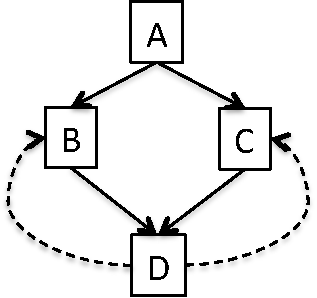
\includegraphics[width=0.5\textwidth]{figs/dependenceGraph.pdf}
\end{minipage}


&

\begin{minipage}[b]{4.25cm}
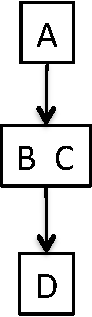
\includegraphics[height=0.15\textheight]{figs/MPCloop.pdf}
\end{minipage}

&

\begin{minipage}[b]{4.25cm}
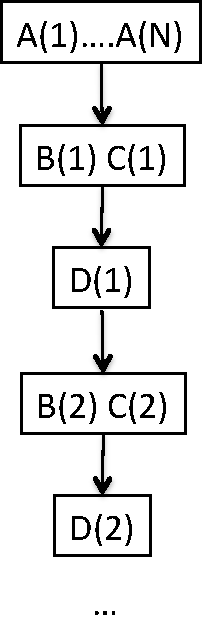
\includegraphics[height=0.20\textheight]{figs/MPCaccrossLoop.pdf}
\end{minipage}
\\


(a) Source 
&
(b) Dependence graph
&
(c) Loop-body schedule
&
(d) Across-loop schedule

\end{tabular}
\caption{(a) shows the source code, taken from Aiken and Nicolau~\cite{Aiken:1988}, 
(b) shows the dependence graph. The solid edges denote within-iteration ordering constraints, e.g., A must run before B
because B depends on A. The dashed edges denote across-iteration ordering constraints, e.g., B(2), i.e., B in iteration 2
depends on D(1), i.e., D in iteration 1. (c) shows the optimal loop-body schedule, and (d) shows the
optimal across-loop schedule. A(1), B(1), etc. denote instruction A in iteration 1, etc.}
\label{fig:MPCexample}\vspace{-2ex}
\end{figure*}

\paragraph{Problem 2:} Given a dependence graph of MPC instructions representing a loop body (or given a loop-body schedule), 
find the \emph{across-loop} schedule with  \emph{minimal cost}.

\figref{fig:MPCexample} illustrates the problem with a code example from the classical high-performance computing (HPC) literature. 
\figref{fig:MPCexample}(c) shows the optimal loop-body schedule (answer to Problem 1). Instructions B and C can be scheduled in parallel, 
however, the schedule does not necessarily benefit form parallelization/amortization. If B and C (functions $f_1$ and $f_2$) are the \emph{same}
MPC instruction (e.g., both are MUX, MUL, ADD, or CMP, etc.), then they \emph{can} benefit from parallelization/amortization. Given
our assumptions stated above, the cost of running the loop-body schedule is 3. However, if B and C are different MPC-instructions,
e.g., B is MUL, but C is MUX, then the cost of running the schedule is 4. 

\figref{fig:MPCexample}(d) shows the optimal across-loop schedule (answer to Problem 2). We can schedule all A-instructions, across all iterations, 
in parallel, as A depends only on the initial value of B. We cannot do better but schedule B, C, and D sequentially, as they each depend on values
computed in the previous iteration. Again, if B and C are the same instruction, the optimal across-loop schedule will have cost of $1 + 2N$, 
and if B and C are NOT the same instruction, then it will have cost $1+3N$.







\section{Scheduling in HPC}

In this section, we state the classical HPC scheduling problem, and argue the MPC scheduling problem poses unique challenges.

Similar problems arise in the HPC setting.

%\begin{figure*}[tbhp]
\begin{figure*}[tbhp]
\begin{tabular}{lll}


\begin{minipage}[b]{4.25cm}
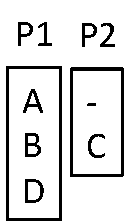
\includegraphics[width=0.4\textwidth]{figs/HPCloop.pdf}
\end{minipage}

&

\begin{minipage}[b]{4.25cm}
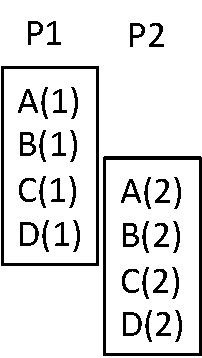
\includegraphics[width=0.4\textwidth]{figs/HPCdoacrossLoop.pdf}
\end{minipage}

&

\begin{minipage}[b]{4.25cm}
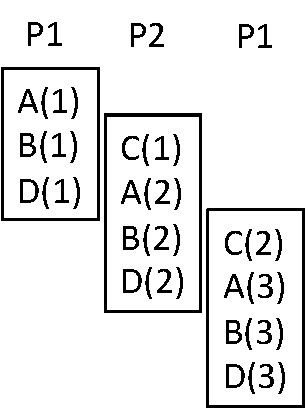
\includegraphics[width=0.6\textwidth]{figs/HPCgreedyLoop.pdf}
\end{minipage}

\\

(a) Loop-body schedule
&
(b) Doacross across-loop schedule
& 
(c) Greedy across-loop schedule

\end{tabular}
\caption{Optimal HPC schedules.}
\label{fig:HPCexample}\vspace{-2ex}
\end{figure*}


\paragraph{Problem 1:} Given a loop body (i.e., dependence graph), find the loop-body schedule with \emph{minimal delay}. 

\paragraph{Problem 2:} Given a loop body (or a loop-body schedule), find the \emph{doacross} schedule with minimal delay.

\paragraph{Problem 3:} Given a loop body (or a loop-body schedule), find the \emph{greedy schedule} with minimal delay.

\figref{fig:HPCexample} illustrates the problem in HPC. \figref{fig:HPCexample}(a) shows the optimal loop-body schedule
which results in cost of 3. Again, we assume that all instructions have the same cost, a unit of 1. The key difference with the 
MPC schedule is that regardless of whether B and C are the same instruction opcode or not, B and C can be scheduled 
to run in parallel and the overall running time benefits from parallelization. 

The HPC literature has considered different kinds of across-loop scheduling. One scheduling, called \emph{doacross}~\cite{aiken,cytron},
requires that all instructions in an iteration are scheduled on the same processor. The optimal doacross schedule for our example
is shown in \figref{fig:HPCexample}(b) (taken directly from~\cite{aiken}). Aiken and Nicolau proposed a new schedule,
which they called \emph{greedy} schedule, where instructions in an iteration can be scheduled on different processors. 
The optimal greedy schedule for our example, which achieves better minimal delay than the optimal doaccross schedule, 
is shown in \figref{fig:HPCexample}(c) (again, taken directly from~\cite{aiken}). 

\ana{Here we have to make the argument that MPC is different from HPC.}
The example illustrates that optimal MPC scheduling and optimal HPC scheduling are different problems.




%\section{\bf Preliminaries}
%\label{sec:preliminaries}

\ana{Relevant papers/books: 

\begin{enumerate}

\item Book: "Scheduling and automatic parallelization", Springer 2000, by Alain Darte, Yves Robert and Frederic Vivien. 
This book describes scheduling and parallelization in HPC: given a dependence graph and unlimited 
number of processors, one can compute an optimal (minimal delay) schedule in polynomial time. 
Given a finite number of processors, computing an optimal schedule becomes NP-hard.

\item https://theory.stanford.edu/~aiken/publications/papers/pldi88.pdf. "Optimal loop parallelization", PLDI 1988, by
Alex Aiken and Alex Nicolau. 
Given a dependence graph of the loop body, computes an optimal parallelization across loop iterations. 
The optimality metric is minimal delay. E.g., assuming 2 iterations, the delay is measured by the number 
of instructions in iteration 2 that are lagging behind iteration 1. 

\item https://www.cs.indiana.edu/~achauhan/Teaching/B629/2006-Fall/CourseMaterial/1998-popl-knobe-arrayssa.pdf.
"Array SSA", POPL 1998, by Kathleen Knobe and Vivek Sarkar. This paper defines an SSA form for arrays which I think 
is crucial for parallelization across loop iterations.

\end{enumerate}
}

\section{Loop Body Parallelization}
\label{sec:parallelization_within_loop}
%\section{Loop-body Analysis}
\label{sec:loopbodyanalysis}

We first consider the answer to \problemref{problem:prob1} (in MPC). 
%\ana{Lindsey, you have to define Problem 1. This is the problem to compute the optimal 
%schedule taking into account just intra-loop dependences.}
We argue that optimal parallelization within a loop body is NP-Hard (under the above stated assumptions). 
Therefore, compilers must resort to heuristics to compute a schedule for the instructions within a loop body.

We consider two operations, call them $A$ and $M$. $A$ and $M$ are two abstract MPC instruction, 
but as an example, $A$ stands for the ADD MPC instruction 
and $M$ stands for the MUL instruction. Each instruction in the program is either an $A$-instruction or
an $M$-instruction. In order to benefit from parallelization/amortization, we must schedule two or more 
$A$-instructions in the same parallel node (or two or more $M$-instructions in the same parallel node). 
Scheduling $A$-instructions in parallel with $M$-instruction does not benefit from amortization.
It incurs the exact same cost as scheduling the $A$-instructions in a node $P_A$, scheduling the $M$-instructions 
in a node $P_M$, and having $P_A$ precede $P_M$ in the parallel schedule. This is the difference 
between classical scheduling, as studied in parallel computing, and MPC scheduling. 

In our theoretical treatment, we make the following assumptions:

\begin{enumerate}

\item $A$ and $M$ are of equal cost, 1 unit.
\item There is unlimited bandwidth---i.e., a single $A$-instruction (or $M$-instruction) costs as much as $N$ amortized $A$-instructions 
(or $M$-instructions), namely 1 unit.
 
\end{enumerate}

%  Furthermore the run time cost of 
% computing operations of the same type remains the same regardless of the number of operations that are run.
% Roughly speaking, 1 A operation costs the same as 100 A operations and 1000 A operations. 

Consider a loop body that consists of $n$ sequences: $S_1$, ... $S_n$ of $A$ and $M$ instructions. 
More precisely, the loop body is such that its instructions can be grouped into such sequences. 
$S_1$, ... $S_n$ can execute in parallel, however, all instructions within a sequence must 
execute sequentially. For example, consider the three sequences (the right arrow indicates a \emph{dependence},
meaning that the source node must execute before the target node): 
\begin{enumerate}
\item $A \rightarrow M \rightarrow A$
\item $A \rightarrow A \rightarrow A$
\item $M \rightarrow A \rightarrow M$
\end{enumerate} 

A \emph{schedule} $P: P_1 \rightarrow P_2 \dots \rightarrow P_k$ is such that for each sequence 
$S_i$ in the set, if $S_i[k]$ precedes $S_i[k']$ in $S_i$ then $S_i[k]$ is scheduled in node $P_l$, $S_i[k]$ 
is scheduled in node $P_{l'}$, and $P_l$ precedes $P_{l'}$ in $P$. 

The cost of a schedule $P$ is 

\begin{equation}
\mathit{cost}(P) = \sum_{i=1}^k \mathit{cost}(P_i)
\end{equation}

where $\mathit{cost}(P_i) = 1$ if $P_i$ consists of $A$-instructions only, or $M$-instructions only, 
and $\mathit{cost}(P_i) = 2$ if $P_i$ mixes $A$-instructions and $M$-instructions. 

The problem is to find a schedule $P$ with \emph{minimal cost}. For example, 
a schedule with minimal cost for the sequences above is
\[ A(1), A(2) \rightarrow M(1), A(2), M(3) \rightarrow A(1), A(2), A(3) \rightarrow M(3) \]
(The parentheses above indicate the sequence where the instruction comes from: (1), (2), or (3).)
The cost of this schedule is 5. 

The problem of finding a schedule $P$ with a minimal $cost(P)$ for a given loop body has been shown
to be an NP-Hard problem, as it can be reduced to the problem of finding a \emph{shortest common supersequence}, 
a known NP-Hard problem\cite{Maier1978},\cite{Vazirani2010}. The shortest common supersequence problem is as follows: 
given two or more sequences find the the shortest sequence that contains all of the original sequences. This can be solved
in $O(n^k)$ time, where $n$ is the cardinality of the longest sequence and $k$ is the 
number of sequences. For our problem $n$ is the maximum length of a node and $k$ is the number
of total number of nodes. %\ana{I think it is clear without additional explanation...}
%\ana{Also, add the full statement of the problem here. Now it's not clear what's NP-hard, what's n, what's k, etc.?}
%\lindsey{not exactly sure what need to go it there, but does that make it clearer?}

To see the reduction, 
suppose $P$ is a schedule with minimal cost (computed by a black-box algorithm). 
We can derive a schedule $P'$ with the same cost as $P$, by mapping each mixed node $P_i \in P$ 
to two consecutive nodes in $P'$: an $A$-instruction node followed by an $M$-instruction node.
Clearly, $P'$, which now is a sequence of $A$'s and $M$'s, is a supersequence of each sequence 
$S_i$, i.e., $P'$ is a common supersequence 
of $S_1 \dots S_n$. It is also a shortest common supersequence. (To see this, suppose, a 
shorter common supersequence, $P''$, exists. $P''$ is a schedule of $S_1 \dots S_n$
and the $\mathit{cost}(P'')$ equals the length of $P''$. Since $P'$ is longer than
$P''$, and $\mathit{cost}(P') = \mathit{cost}(P)$, that means $\mathit{cost}(P'') < \mathit{cost}(P)$, 
which is a contradiction since $P$ is a schedule with minimal cost.)

%\ana{Question: are these two assumptions too strong?} \lindsey{I don't think so? makes sense to me}

%\ana{Assumption 1 can be relaxed --- e.g., if $A$ is 5 times cheaper than $M$, 
%we can construct a program where all $A$'s are sequences of five consecutive 
%$A$'s, which reduces to the previous problem.} \lindsey{it doesn't matter I think... as long as it is a static 
%difference.}

%\ana{Assumption 2, I am not sure if this is acceptable, or maybe it is too strong. My intuition is that incorporating into the cost a dependence on the number of instructions in each parallel node, is going to make the problem harder, not easier...} 
%\lindsey{I think that the important note is that it is mannnnny magnitudes of 10 cheaper}
%\lindsey{Ana, Is this now a stale comment?}


\section{Across-loop Analysis}
\label{sec:analysis}

We have shown that in general scheduling a loop body is NP-hard. However, in practice loop bodies consist
of relatively small number of statements. Multiple parallel sequences as in the proofs above, are uncommon.
Therefore, one can compute the shortest common supersequence using a brute force approach. 

In this section, we describe the computation of the across-loop schedule. The algorithm proceeds in several phases. 
First, we extend Cytron et al.'s algorithms, outlined in \secref{sec:ssa}
to construct the MPC-MUX nodes. Even though there is significant overlap between SSA construction 
and translation to MPC target code, the problem of placing MUX nodes has not been previously addressed.
We define an algorithm that addresses this problem in~\secref{sec:cfgtompc}. Second, we handle arrays in a way that
improves parallelization. We describe this handling in~\secref{sec:arrayhandling}. These two parts give rise to a graph where  
each node is an MPC target code statement. The edges represent the intra-loop control flow and largely 
overlap with the original CFG edges. The statements are in SSA form and $\phi$-nodes are replaced with MUX nodes. 
We call this graph the MPC $G$. 

Once we have constructed the MPC $G$ for the loop body, we construct the dependence graph $G$, which reflects
intra-loop dependences and across-loop dependences. We describe the construction of $G$ 
in~\secref{sec:depgraph}. % and~\secref{sec:depgraphalgo}. 
%\ana{Broken link}\lindsey{removed the second one. links to old section of paper that is commented out.}
This graph gives rise of the across-loop schedule, which we describe in~\secref{sec:loopscheduling}. 
%\ana{Lindsey, can you fix these references?}

\subsection{High-level CFG to MPC $G$} 
\label{sec:cfgtompc}

\subsubsection{From $\phi$-nodes to MUX-nodes}

%\ana{Difficulties: Translate to MUX nodes, adapt classical SSA algorithm, arrays, reads and writes!}

% \begin{figure}
% \small
% \[
% \begin{array}{l@{~~~~~}l}
%   \begin{array}{l@{~}l@{~~~}l}
%   s & ::= s ; s \\ 
%   & \mid \x = \y \; \mid \x=\y \; \op \; \z \mid {\sf A[f(i)] = x} \; \mid {\sf x = A[f(i)]} & \mathit{assignment} \\
% %  & \mid \x = \phi(\y,\z) \\
%   & \mid {\sf for} \; (i = 0; i \le \mathit{Const}; \mathit{i\!+\!+}) \; \{ \; s \; \} \\
%   & \mid {\sf if} \; (\x \; \cop \; \y) \; \{ \; s \; \} \; {\sf else} \; \{ \; s \; \} \\
%  % \bool &::= \x \; \cop \; \y & \mathit{comparison} \\
%   \op &::= + \mid - \mid * \mid / & \mathit{arithmetic} \; \mathit{operator} \\
%   \cop &::=  \; == \; \mid \; != \; \mid \; < \; \mid \; \le & \mathit{comparison} \; \mathit{operator}

%   \end{array}
% \end{array}
% \]
% %\vspace{-0.2in}
% \caption{IMP syntax as defined in \cite{Ishaq2019}: $s$ is a sequence of statements. 
% \code{x}, \code{y}, \code{z}, and $i$, are variables. \ana{Remove Fig. 16 because you have Fig. 14. But take f(i) for array indices in 14.}
% } 
% \label{fig:syntax}
% \end{figure}


Again, we consider a standard IMP-like\cite{Nipkow2014} imperative language.
Without loss of generality, we assume that the syntax gives rise to a CFG and we can apply the 
Cytron et al.'s Algorithm for the efficient computation of SSA over this CFG~\cite{Cytron1991}
(shown in \algref{alg:cytronphiplacement} and \algref{alg:cytronlabeling}). 

% Once we have the code in 
% SSA form with we can proceed to transform if statements into MUX nodes.

\begin{figure}[h]
\centering
\begin{minipage}{0.7\textwidth}
\begin{javacode}
z = 0;
...
if (x > 0) {
  if (y > 0) {
    z = 1;
  }  else {
    z = -1;
  }
}
print(z);
\end{javacode}
\end{minipage}
\caption{Branching Code.}
\label{fig:examplecfgcode}
\end{figure}

In particular, we are interested in a sequence of statements that form a loop body, i.e., while 
the outermost statement is a {\sf for} the remaining statements are assignments and {\sf if}s.
There are two principal hurdles. One is to translate the CFG into SSA form, where $\phi$ nodes 
are turned into MUX nodes. One cannot simply reuse the classical algorithm by Cytron et. al. 
because $V_3 = \phi(V_1,V_2)$ nodes do not retain information about the predicate that triggers 
$V_1$ vs. $V_2$; all $\phi$ nodes represent is conditional control flow, i.e., that $V_3$ is either 
$V_1$ or $V_2$. Another issue is that SSA $\phi$ nodes can combine multiple conditionals. 

\begin{figure}[H]
\centering
\begin{minipage}{0.30\textwidth}
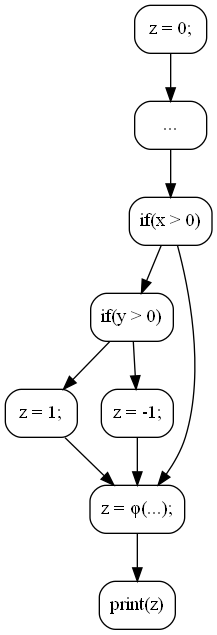
\includegraphics[width=\textwidth]{cfgphinode}    
\end{minipage}
\caption{CGF after \algref{alg:cytronphiplacement} is run.
The $\phi$ node is added but no labeling has taken place.}
\label{fig:cfgwithphinode}
\end{figure}

\begin{figure}[H]
\centering
\begin{minipage}{0.38\textwidth}
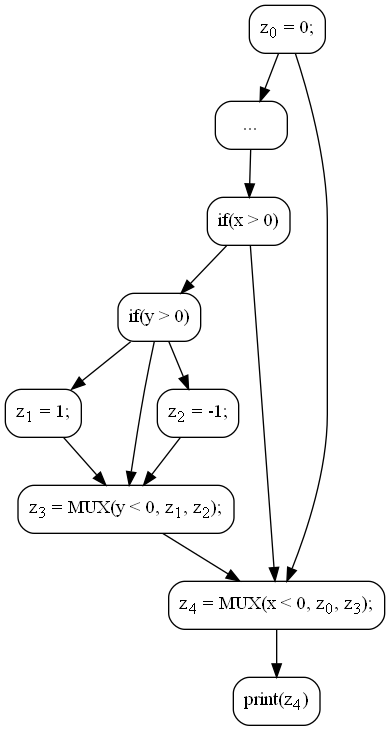
\includegraphics[width=\textwidth]{cfgmuxnode}    
\end{minipage}
\caption{Result of running \algref{alg:cytronextension}. 
MUX nodes are added at merges and refer to conditionals.}
\label{fig:cfgwithmuxnode}
\end{figure}

To illustrate, consider the code shown in \figref{fig:examplecfgcode}.
Line 10 is the dominance frontier of the assignments to 
\z, and Cytron et. al.'s algorithm creates a $\phi$ node at 10: $z_3 = \phi(z_0, z_1, z_2)$. 
There is no information retained that $z_0$ is triggered when $x \le 0$, $z_1$ is triggered when 
$x > 0 \; \wedge \; y > 0$, and $z_2$ is triggered when $x > 0 \; \wedge \; y \le 0$. The Multiplexer at the join point
needs this information in order to assign the correct value to $z_3$ at runtime.

We propose a simple extension to the classical algorithm. Recall from Cytron et. al.'s 
that efficient static single assignment computation has two phases, phase one is the 
placement of phi-nodes at dominance frontiers of assignments, and phase two is the 
renaming of variables $V$ into $V_1$, $V_2$, etc. \figref{fig:cfgwithphinode}
shows the CFG after \algref{alg:cytronphiplacement} is run. The $\phi$ node is placed but the 
variables have not been labeled correctly. Instead of transforming the phi node completley
we instead create MUX nodes that reference the conditionals that are associated with each variable.
MUX nodes are then placed at the merge points as shown in, and all the variables are labeled,
\figref{fig:cfgwithmuxnode} shows the CFG after this step. The algorithm for this 
extension is shown in \algref{alg:cytronextension}. 

%\lindsey{changed font size in algo to footnotesize.... is that too small?} \ana{It's good.}
\begin{algorithm}
\footnotesize
\begin{algorithmic}[1]
\ForAll {variables $V$}
\State $C(V) \leftarrow 0$
\State $S(V) \leftarrow \mathit{EmptyStack}$
\State $P \leftarrow \mathit{EmptyStack}$
\EndFor
\State call SEARCH($\mathit{Entry}$) \\
\State ... \\
SEARCH(X) : \\
\ForAll {statements $A$ in $X$} 
\If {$A$ is a $\phi$-assignment}
   \State {remove $A$ and continue}
\EndIf
\ForAll {variables $V$ in $\mathit{RHS}(A)$}
   \State {replace $V$ with $V_i$ where $i = \mathit{Top}(S(V))$}
\EndFor

\ForAll {variable $V$ in $\mathit{LHS}(A)$}
   \State { $i \gets C(V)$} 
   \State {replace $V$ with $V_i$ in $\mathit{LHS}(A)$}
   \State {push $i$ onto $S(V)$}
   \State {$C(V) \gets i+1$}
\EndFor
\EndFor
\ForAll {$Y \in Succ(X)$}
\If {$X$ is a conditional node}
   \State {push $\mathit{Cond}, \mathit{Branch}$ onto $P$ // $\mathit{Branch}$ is $T$ if $X \rightarrow Y$ is the True branch, $F$ otherwise}     
\EndIf   
     \State{// $Y$ is not done if $Y$ has an incomplete MUX predecessor or an original CFG predecessor}
      \If {$Y$ has $\phi$-assignments and $Y$ is not done} 
          \State {$\mathit{Cond}, \mathit{Branch} \gets$ pop $P$}
          \ForAll {$\phi$-assignments in $Y$}
               \If {$Z\!: V = \mathit{MUX}(Cond, ..., ...) \in \mathit{Pred}(Y)$}
                  %\STATE {replace $V$ in $RHS(Z)$ with $V_i$, where $i = Top(S(V)$}
                  \State {remove edge $X\rightarrow Y$, add edge $X\rightarrow Z$ to $\mathit{CFG}$}
                  \State {call SEARCH($Z$) // updates $V$'s in LHS and RHS} 
               \Else
                   \State {$i = Top(S(V))$}
                   \If {$\mathit{Branch} == T$}
                      \State {create new node $Z\!: V = \mathit{MUX}(\mathit{Cond}, V_i, V)$}
                   \Else 
                      \State {create new node $Z\!: V = \mathit{MUX}(\mathit{Cond}, V, V_i)$}
                   \EndIf   
                   \State {remove edge $X\rightarrow Y$, add edge $X\rightarrow Z$ to $\mathit{CFG}$} 
               \EndIf
          \EndFor 
      \EndIf
\EndFor
\ForAll {$Y \in \mathit{Children}(X)$}
   \State {call SEARCH($Y$)}
\EndFor
\ForAll {assignments $A$ in $X$}
   \ForAll {variables $V$ in oldLHS($A$)}
       \State {pop S(V)}
   \EndFor
\EndFor
\end{algorithmic}
\caption{Extension of \algref{alg:cytronphiplacement} replacing $\phi$ nodes with MUX nodes}
\label{alg:cytronextension}
\end{algorithm}

%\lindsey{Ana, I think I got it now! Check the figures!} \ana{Yes, excellent!}
% \ana{TODO: Ana: Here we need an explanation for lines 23-45. Turning n-ary phi-nodes into binary MUX nodes, 
% just the same classical algorithm with minor extension.} \lindsey{which lines/figure?}\ana{Lines in the Algo. I'll do it.}
% \ana{TODO: Lindsey: Example of CFGs for above example.} \lindsey{I made the CFG.... but am still confused, there
% are only 10 lines in the example?} \ana{Yes, that one's almost there. But this is the MUX graph, each MERGE becomes a MUX.}
% \ana{This graph is the After graph, with each MERGE node now a MUX node. In the after graph, show the MUX what arguments it takes.} 
% \ana{We also need the Before graph which has just a single Dominance Frontier node that merges control from all the conditionals.}
% \lindsey{now I am really confused.... how many graphs should there be?}

\subsubsection{Handling of Arrays}
\label{sec:arrayhandling}

So far we focused on the classical SSA analysis and the extension to create MUX nodes. 
Classical SSA treats arrays as scalars, i.e., an array write, e.g., {\sf A[i] = x+y} is considered
a modification of {\sf A} and warrants its own indexed variable ${\sf A}_k$. A later use of {\sf A}, 
even one such as {\sf x = A[i+1]} where there is no def-use link from {\sf A[i] = x+y}, will be 
considered a use of ${\sf A}_k$. This hinders parallelization. To illustrate, consider 
what is shown in \figref{fig:arrayhand}.
%\begin{minted}[fontsize=\footnotesize, numbersep=5pt, escapeinside=||]{java}

\begin{figure}[H]
\centering
\begin{minipage}{0.7\textwidth}
\begin{javacode}
for (...) {
  A: A[i] = f_1(B[i]);
  B: B[i] = f_2(A[i]);
  ...
}
\end{javacode}
\end{minipage}
\caption{Array handling.}
\label{fig:arrayhand}
\end{figure}

%\end{minted}
Since {\sf A} and {\sf B} are treated as standard scalars, the dependence analysis will record
a dependence from {\sf B} to {\sf A} via the back edge. As a result, statement {\sf A} wouldn't 
be vectorized because each (i+1)-th iteration depends on {\sf B} in the i-th iteration,
which depends on {\sf A} in the i-th iteration. 

To mitigate against this, we propose a technique, similar to Array-SSA though much simpler and 
less general, which breaks certain dependence edges and allows for better vectorization. 
We term this technique \emph{scalar substitution}.
%\ana{Have to make a claim how often this technique resolves dependences perfectly, and how often it defaults to standard SSA.}

%\ana{TODO: Summary of the technique}

The essence of scalar substitution is that in certain cases, one can treat array accesses as distinct scalar accesses.
For example, reads and writes of $\A[i]$ are treated as reads and writes to a scalar variable $\A[i]$.
Our SSA transformation assigns versions $\A[i]_0$, $\A[i]_1$, etc. when $\A[i]$ is written in the loop body. 
The key issue is that we need to properly account for across-loop dependences. When there is an array write 
$\A[f(i)] = ...$ and an array read $ ... = \A[f'(i)]$ and the array references have been replaced with scalar variables, 
our analysis must properly account for across-loop dependences from one scalar variable to another.

In summary, our technique first outlines conditions on arrays that will allow us to safely carry such transformation.
These are the Array Well-formedness conditions defined below. If these conditions hold for array \A, then when 
we do scalar substitution for \A: we replace 
array accesses of {\A} with scalars. Otherwise, we leave {\A} as is, defaulting to the standard treatment in Cytron et al. 
The standard treatment treats writes to different indices of {\A} as writes to a single variable {\A}, and similarly, reads
to different indices of {\A} as reads of that single variable. This is safe, however, it may miss opportunities for
parallelization. In our experience, our Array Well-formedness conditions are not restrictive, as in the majority of benchmarks
(typical MPC benchmarks), arrays are read-only. However, more experiments are needed, particularly 
with benchmarks that are standard in HPC, that we hope to transfer to our setting. 

Our technique next constructs the dependence graph taking into account the replacement with scalar variables. 
This is described in~\secref{sec:depgraph}. The algorithm constructs a correct dependence graph taking into 
account loop-carried dependences between scalars in the cases when Array Well-formedness holds.

\paragraph {Equivalence and Non-equivalence} Let $f(i)$ and $f'(i)$ be two index functions on induction variables $i$, 
e.g., we have array accesses ${\A}[f(i)]$ and ${\A}[f'(i)]$. We say that $f(i) \cong f'(i)$ iff for every $1 \le i \le N$,
$f(i) = f'(i)$. We say that $f(i) \ncong f'(i)$ iff for every $1 \le i \le N$, $f(i) \neq f'(i)$. 
%\ana{TODO Ana. This needs to be expanded
%with consideration of equivalence classes of variables in f(i). 
%For some set of variables functions are equivalent for another set they are non-equivalent, etc.
%Have to say something, for a fixed set of constants...}

Strictly, equivalence and nonequivalence is defined under conditions on variables in $f(i)$ and $f'(i)$ 
other than the induction variable $i$. For example if $f(i) = x*i$ and $f'(i) = x*(i-1)$, equivalence and non-equivalence 
depends on $x$. If $x$ is 0 then the two formulas are equivalent and if $x \neq 0$ then they are non-equivalent. 
When we write $f(i) \cong f'(i)$ we mean that the following logical formula is valid:

\begin{equation}
1 \le i \le N \Rightarrow f(i) = f'(i) 
\end{equation}
and similarly, 
\begin{equation}
1 \le i \le N \Rightarrow f(i) \neq f'(i) 
\end{equation}
In future work we will consider conditional equivalence and non-equivalence, i.e, in the above example, we will 
consider formulas
\begin{equation}
x = 0 \Rightarrow (1 \le i \le N \Rightarrow f(i) = f'(i)) 
\end{equation}
and
\begin{equation}
x \ne 0 \Rightarrow (1 \le i \le N \Rightarrow f(i) \neq f'(i) ) 
\end{equation}

\paragraph{Array Well-formedness Conditions} Let ${\A}$ be an array mentioned in the loop body. 
We will treat array accesses ${\A}[f(i)]$ as distinct scalar variables if we can show that the loop body is
well-formed with respect to \A. Otherwise, we treat array {\A} as a single variable, thus defaulting to the 
case of standard SSA. The array well-formedness conditions for array {\A} are defined as follows: 

\begin{enumerate}
\item For each pair of array writes to \A, $n_1\!: \A[f(i)] = ... $ and $n_2\!: \A[f'(i)] = ... $, we have either $f(i) \cong f'(i)$ or 
$f(i) \ncong f'(i)$. 

\item In addition, for each pair of array writes to \A, $n_1\!: \A[f(i)] = ... $ and $n_2\!: \A[f'(i)] = ... $, there does not exist 
a pair $1 \le i, j \le N$, $i \neq j$ such that $f(i) = f'(j)$, or in other words array writes are disjoint, i.e., the same array location 
cannot be written in two different iterations. 
%\ana{Check whether one of these is sufficient.}

\item For each pair $n_1\!: \A[f(i)] = ... $ and $n_2\!: ... = \A[f'(i)]$ such that $n_1$ reaches $n_2$ on a forward path, 
we have either $f(i) \cong f'(i)$ or $f(i) \ncong f'(i)$. 

%\item For each pair $n_1\!: A[f(i)] = ... $ and $n_2\!: A[f'(i)] = ... $ either $f(i-d) \cong f'(i)$ for some unique $d > 0$, 
%or $f(i-d) \ncong f'(i)$ for every $d > 1$. 

\item For each pair $n_1\!: \A[f(i)] = ... $ and $n_2\!: ... = \A[f'(i)]$ %such that $n_1$ reaches the loop exit (we assume that there is
%a unique loop exit node) on a forward path, and there is  $n_2$ on a forward path, 
we have either $f(i-d) \cong f'(i)$ for some unique $d$ s.t. $1 \le d < N$, or $f(i-d) \ncong f'(i)$ for every $d$ s. t. $1 \le d \le N$. 

In this $d$ is the distance between the iterations in the loops i.e. For if statement A has a $d$ value of 2 from statement B, 
statement A was computed 2 loop iterations before statement B.

\end{enumerate}

To see the intuition behind these rules, consider rule (1). 
In other words, the two array writes are either equivalent, i.e., at each iteration they modify the same
location, or they are non-equivalent, i.e., at each iteration they modify distinct locations. Note that the two array writes
``clash'' in one way or another. If $n_1$ reaches $n_2$ (or vice versa, $n_2$ reaches $n_1$), then if $f(i)$ and $f'(i)$ 
are neither equivalent nor non-equivalent, there would be a kill in some iterations and not in others; in contrast, if
they are equivalent, there is always a kill, and if they are non-equivalent, there is never a kill. If neither $n_1$ reaches
$n_2$ nor the other way around, then the two array writes will ''clash'' at a join node. If $f(i)$ and $f'(i)$ are neither 
equivalent nor non-equivalent, then there would be one kind of MUX for certain iterations and a different kind of MUX 
for the rest; if $f(i)$ is equivalent to $f'(i)$, then the MUX will be $... = \mathit{MUX}(\mathit{cond}, {\A}[f(i)], {\A[f'(i)]})$, and 
$f(i)$ and $f'(i)$ are non-equivalent then there will be two MUX nodes: $... = \mathit{MUX}(\mathit{cond}, {\A}[f(i)], {\A'[f(i)]})$
and $... = \mathit{MUX}(..., {\A}[f'(i)], {\A'[f'(i)]})$. (Note that after SSA, the A's will be properly indexed.)
%\ana{I need explanations of (2) and (3).} 

Condition (2), disjointness of writes, is necessary for our graph construction algorithm to properly account
for loop-carried dependences. We have to make sure that a write in a later iteration $i$ does not ''kill'' a write in an earlier iteration $j$.

Similarly, for (3) if an array write reaches an array read they either reference 
the same location or never reference the same location. In other words, there is either an intra-loop 
def-use in each iteration, or there is no intra-loop def-use in any iteration. 
More concretely if we have $A[f(i)] = ...$ flow into $... = A[g(i)]$ then for $1 \le i \le N, f(i) = g(i) ~ | ~ \mbox{ for } 1 \le i \le N, f(i) \neq g(i)$. 

Finally, (4) is a little more involved, if there is an array write and then a read and they always differ, 
they always differ by a static constant $d$. This would mean that the read always uses the write $d$ iterations before.
%So then if we again have $A[f(i)] = ...$ flow into $... = A[g(i)]$ and 
%$\forall i \in \Z, f(i) \neq g(i)$ then $\forall i \in \Z, f(i) - g(i) = d$ where $d \in \Z$. \lindsey{Ana, doe this make sense}


\paragraph{Example} Consider our running example in \figref{fig:arrayloop}. 
There is a single write to each array in the loop body,  so there are no write-write pairs and no 
tests for (1). There are the following write-read pairs: 2 and 3 (access of \A), 
2 and 4 (access of \A), 3 and 5 (access of \B), 4 and 5 (access of \C), 3 and 2 (access of \B), 5 and 3 (access of \D) 
and 5 and 4 (access of \D).
We apply the forward test, (2), only on the first three pairs, as for the remaining ones, there is no forward path from 
the write to the read. 
Test (2) clearly passes because $i$ is obviously equivalent to $i$. For the remaining pairs, we only apply the backward 
test, test (3). 
Pair 3 and 2 passes as well because $i-1$ and $i$ are nonequivalent for every $d > 0$. 5 and 3, and analogously 5 and 
4, pass test (3). 
In these two cases, the unique $d = 1$ makes $i - d$ and $i-1$ equivalent. 

\paragraph{Checking well-formedness}

%\ana{TODO Ana: Add paragraph on checking.}

We ensure the above conditions as follows:
For conditions 1. and 3. we check the validity of the following formula: 
\begin{equation}
(1 \le i \le N \Rightarrow f(i) = f'(i)) \vee (1 \le i \le N \Rightarrow f(i) \neq f'(i))
\end{equation}
For condition 2 we check validity of
\begin{equation}
(1 \le i,j \le N \wedge i\neq j \Rightarrow f(i) \neq f'(j))
\end{equation}
Finally, for condition 4 we find $d$ by asking satisfiability of
\begin{equation}
1 \le i \le N \Rightarrow f(i-d) = f'(i)
\end{equation}
and then ensure validity of
\begin{equation}
1 \le i \le N \wedge 1 \le d' < N \wedge d' \neq d \Rightarrow f(i-d) \neq f'(i)
\end{equation}

This checks can be done with off the shelf SMT solvers such as Z3. 


%\ana{Where do we put this? Theorem: simple rule is not restrictive} \ana{This one can be left out.}
%\ana{TODO Ana: Theorem 2: program is equivalent to transformed one where each A[f(i)] is replaced with a scalar.}  
%\ana{The idea is that we replace each A[f(i)] with scalar, i.e., we treat A[f(i)] like a scalar. E.g., if we have A[i] in our SSA algorithms we are treating it as $A_i$ , a variable. We'll compute versions of Ai like Ai_1, Ai_2, etc., just like for scalars.} 
%\lindsey{I think we cover this above now? Is this a stale comment?}


\subsection{Across-loop Dependence Graph $G$: Overview}
\label{sec:depgraph}

Our next step is to determine dependences, including intra-loop dependences and more complex 
across-loop dependencies through the creation of the dependence graph $G$ and analysis and 
reasoning over $G$. Our transformation analyzes arrays as described earlier, and does scalar substitution
for well-formed arrays, while treating non-well-formed arrays in the standard way. Then we use \algref{alg:cytronextension}
on the loop body code to add MUX nodes. 

Each node of the $G$ represents an MPC target code statement in a loop body, while each edge
represents a def-use dependency between the two connected nodes. The analysis considers
each statement of the loop. If the statement contains an array reference (Note, 
that SSA guarantees that there can be only one array reference in any single
statement) it is classified as a read, or a write. The statement is a write only
if the statement is an assignment statement, and the array reference is on
the left-hand side of the assignment, otherwise it is classified as a read.
This statement, its original source line number, and index of the array
reference are stored as a node. Scalars that change per iteration are also
handled. Every scalar that changes in the loop body is defined in a $\phi$
node at the head of the loop, and the changed variable is defined
at the end of the loop. This makes tracing reads and writes of 
changing variables as easy as tracing induction variables through the loop
and noting the node that defines the changed variable.
%\ana{Lindsey, you talk about array references, but how about scalar reads and writes?}
%\lindsey{not explained perfectly, work in progress, but does that make more sense?}
%\ana{Somewhere here we need to say that we apply Alg. 3 to produce the SSA.}
%\lindsey{blunt, but effective? Is that OK?}

%\ana{This was repeated from above, removed.}
%Each node of the SCC represents a statement in a loop body, while each 
%edge represents a dependency between the two connected nodes. The parser 
%analyzes each statement of the loop. If the statement contains an array 
%reference (Note, that SSA guarantees that there can be only one array reference 
%in any single statement) it is classified as a read, or a write. The statement 
%is a write only if the statement is an assignment statement, and the array reference 
%is on the left-hand side of the assignment, otherwise it is classified as a read. 
%This statement, its original source line number, and index of the array 
%reference are stored as a node.

After all the nodes have been found, edge creation and labeling begins. 
For each node, $c$, in the graph the following steps are taken to determine 
the distance between each pair of def/use statements. This value determines 
the parallelization schedule for each pair interaction 
in the context of the larger loop body. The full algorithm is shown in 
\algref{alg:edgecreation}.

\begin{algorithm}
\begin{algorithmic}
\State // Step 1: Forward edge construction 
\ForAll{$n_1 \in \mathit{Nodes}(G)$}
\ForAll{$n_2 \in \mathit{Nodes}(G)$}
\If{$n_1 \neq n_2$}
\ForAll{$v \in \mathit{Scalars}(G)$}
%\State $MaxNode \leftarrow GetMaxNodeScalar(v)$
\If{$v \in \mathit{LHS}(n_1)$ \&\& $v \in \mathit{RHS}(n_2)$}
\State $\mathit{Edges} \leftarrow \mathit{Edges} \cup \mathit{ForwardEdge}(n_1, n_2)$
\EndIf
\EndFor
\ForAll{$\A \in \mathit{Arrays}(G)$}
\If{$\A[f(i)] \in \mathit{LHS}(n_1)$ \&\& $\A[f'(i)] \in \mathit{RHS}(n_2)$ \&\& $f(i) \cong f'(i)$} %$\forall i \in \Z, f(i) == f'(i)$}
\State $\mathit{Edges} \leftarrow \mathit{Edges} \cup \mathit{ForwardEdge}(n_1, n_2)$
\EndIf
\EndFor
\EndIf
\EndFor
\EndFor
\State // Step 2: Backward edges for scalars (including non well-formed arrays)
\ForAll{$v \in \mathit{Scalars}(G)$}
\State $\mathit{MaxNode} \leftarrow \mathit{GetMaxNodeScalar}(v)$
\ForAll{$n \in \mathit{Nodes}(G)$}
\If{$n \neq \mathit{MaxNode}$ \&\& $V_0 \in \mathit{RHS}(n)$}
\State $\mathit{Edges} \leftarrow \mathit{Edges} \cup \mathit{BackwardEdge}(\mathit{MaxNode}, n, -1)$
\EndIf
\EndFor
\EndFor
\State // Step 3: Backward edges for well-formed arrays
\ForAll{$\A \in \mathit{Arrays}(G)$}
\State $\mathit{MaxNode} \leftarrow \mathit{GetMaxNodeArray}(\A)$
\State $f(i) \leftarrow \mathit{ArrayWriteIndex}(\mathit{MaxNode})$
\ForAll{$n \in \mathit{Nodes}(G)$}
\If{$\mathit{IsArrayRead}(n)$ \&\& $n \neq \mathit{MaxNode}$ \&\& $A_0 \in \mathit{RHS}(n)$}
\State $f'(i) \leftarrow \mathit{ArrayReadIndex}(\mathit{MaxNode})$
\State $d \leftarrow \mathit{Z3}(f(i), f'(i))$
\State $\mathit{Edges} \leftarrow \mathit{Edges} \cup \mathit{BackwardEdge}(\mathit{MaxNode}, n, d)$
\EndIf
\EndFor
\EndFor
%\EndFor
\end{algorithmic}
\caption{Edge Creation}
\label{alg:edgecreation}
\end{algorithm}

%\ana{The above text is good, we may make some edits later on.}

The following constructs are used in the algorithm

\begin{itemize}
	\item $\mathit{Edges}$ is a set of edges
	\item $\mathit{Nodes}(G)$ returns all nodes in the graph $G$
	\item $\mathit{Scalars}(G)$ returns all scalars in the program including non-well-formed arrays
	\item $\mathit{Arrays}(G)$ returns all well-formed arrays
	\item $\mathit{IsArrayWrite}(N)$ returns true iff $\mathit{LHS}(N)$ is an array write
	\item $\mathit{ArrayWriteIndex}(N)$ returns an index $f(i)$ in an array write, where $i$ is the induction variable
	\item $\mathit{ArrayReadIndex}(N)$ returns an index $f(i)$ in an array read, where $i$ is the induction variable
	\item $\mathit{GetMaxNodeScalar}(V)$ returns a node $N$ such that $V_{\mathit{max}} \in N$
	\item $\mathit{GetMaxNodeArray}(A_{\mathit{max}})$ returns a node $N$ such that $A_{\mathit{max}} \in \mathit{LHS}(N)$
	\item $\mathit{ForwardEdge}(N_1, N_2)$ returns a new node between $N_1$ and $N_2$
	\item $\mathit{BackwardEdge}(N_1, N_2, d)$ returns a new node between $N_1$ and $N_2$ with a distance of $d$
	\item $\mathit{Z3}(f(i), g(i))$ returns the distance $d$ between two indices based on the induction variable $i$
\end{itemize}



%%% DO NOT DELETE! OLD VERSION THAT IS CORRECT!

% \begin{algorithm}
% \begin{algorithmic}
% \ForAll{$n_1 \in Nodes(G)$}
% \ForAll{$n_2 \in Nodes(G)$}
% \If{$n_1 \neq \n_2$}
% \ForAll{$v \in Scalars(G)$}
% \If{$v \in LHS(n_1)$ \&\& $v \in RHS(n_2)$}
% \State $Edges \leftarrow Edges \cup ForwardEdge(n_1, n_2)$
% \EndIf
% \EndFor
% \ForAll{$a \in Arrays(G)$}
% \If{$a[f(i)] \in LHS(n_1)$ \&\& $a[f'(i)] \in RHS(n_2)$ \&\& $\forall i \in \Z, f(i) == f'(i)$}
% \State $Edges \leftarrow Edges \cup edge(n_1, n_2)$
% \EndIf
% \EndFor
% \EndIf
% \EndFor
% \EndFor
% \ForAll{$v \in Scalars(G)$}
% \State $MaxNode \leftarrow GetMaxNodeScaler(v)$
% \ForAll{$n \in Nodes(G)$}
% \If{$n \neq MaxNode$ \&\& $V_0 \in RHS(n)$}
% \State $Edges \leftarrow Edges \cup BackwardEdge(MaxNode, n, -1)$
% \EndIf
% \EndFor
% \EndFor
% \ForAll{$a \in Arrays(G)$}
% \State $MaxNode \leftarrow GetMaxNodeArray(a)$
% \State $f(i) \leftarrow ArrayWriteIndex(MaxNode)$
% \ForAll{$n \in Nodes(G)$}
% \If{$IsArrayWrite(n)$ \&\& $n \neq MaxNode$ \&\& $A_0 \in RHS(n)$}
% \State $f'(i) \leftarrow ArrayReadIndex(MaxNode)$
% \State $d \leftarrow Z3(f(i), f'(i))$
% \State $Edges \leftarrow Edges \cup BackwardEdge(MaxNode, n, d)$
% \EndIf
% \EndFor
% \EndFor
% \end{algorithmic}
% \caption{Edge Creation}
% \label{alg:edgecreation}
% \end{algorithm}

%%% DO NOT DELETE! OLD VERSION THAT IS CORRECT!
\begin{figure}[h]
\centering
\begin{minipage}{0.7\textwidth}
\begin{javacode}
     label1:
        i13_1 = Phi(i13 #0, i13_2 #1);
        if i13_1 > b0 goto label2;
        $i1 = r3[i13_1];
        r1[i13_1] = $i1;
        $i4 = r1[i13_1];
        $i2 = i13_1 - 1;
        $i3 = r7[$i2];
        $i5 = $i4 * $i3;
        r3[i13_1] = $i5;
        $i8 = r1[i13_1];
        $i6 = i13_1 - 1;
        $i7 = r7[$i6];
        $i9 = $i8 * $i7;
        r5[i13_1] = $i9;
        $i11 = r3[i13_1];
        $i10 = r5[i13_1];
        $i12 = $i11 * $i10;
        r7[i13_1] = $i12;
        i13_2 = i13_1 + 1;
(1)     goto label1;
\end{javacode}
\end{minipage}
\caption{Transformed loop body from \figref{fig:arrayloop}.} 
\label{fig:transformedaikenexample}
\end{figure}

\begin{figure}[h]
\centering
\begin{minipage}{0.7\textwidth}
\begin{pythoncode}
from z3 import *
# i2 = i13_1 - 1
# i3 = r7[i2]
i2 = Int('i2')
i13_1 = Int('i13_1')
F = [i2 != 0, i13_1 != 0]
s = Solver()
s.add(F)
s.add(i2 == i13_1 - 1)
print(s.check())
if s.check() == z3.sat:
    m = s.model()
    for el in m:
        print(el, m[el])
\end{pythoncode}
\end{minipage}
\caption{Example of Z3 solving for a $d$ value in \figref{fig:transformedaikenexample}.}
\label{fig:z3example}
\end{figure}

As an example of Z3 solving for a $d$ value consider the code in \figref{fig:z3example}.
This code determines a $d$ value for one of the array accesses in our running 
example taken from Aiken et. al \cite{Aiken1988} and shown in~\figref{fig:arrayloop}. 
% The original equation defining an index variable is flattened and all 
% non-induction variables on the right hand side of the equation are replaced with their induction 
% definitions. \ana{I'm not quite sure what you mean here, can you expand/rewrite?} 
In this case the index variable $i2$ is comparted with a its definition $i13\_1 - 1$ where 
$i13\_1$ is an induction varaible that changes every loop iteration. From this we can create an equation to 
determine distance between the index variable we are interested in (in this case $i2$) and other 
and the induction variable (in this case $i13\_1$). Z3 then finds the smallest possible values that 
to satify this equation. By taking the difference of the generated values we determine the $d$ value (in
this case $d = -1$). 

We also assume the \emph{constant rate assumption} for every statement that we analyze. This ensures
that any one statement cannot have differing d-values regardless of the number of array accesses on the 
right hand side of the assignment. Line 6 in \figref{fig:fibconstantrate} violates this assumption,
as it simultaneously has a d-values of 1 and 2. In other words, the statement at line 6 depends on itself
1 iteration ago and 2 iterations ago. 

\begin{figure}[h]
\centering
\begin{minipage}{0.7\textwidth}
\begin{javacode}
int fib(int n) {
    int[] arr = new int[n];
    arr[0] = 1;
    arr[1] = 1;
    for(int i = 2; i < n; i++) {
        arr[i] = arr[i - 1] + arr[i - 2];
    }
    return arr[n - 1];
}
\end{javacode}
\end{minipage}
\caption{The dynamic program solution for solving the $n$-th Fibonacci number violates the Constant Rate
assumption.}
\label{fig:fibconstantrate}
\end{figure}

\begin{figure}[h]
\centering
\begin{minipage}{0.50\textwidth}
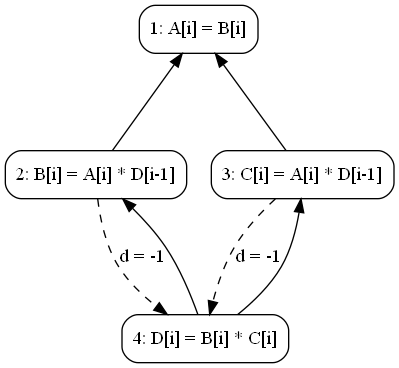
\includegraphics[width=\textwidth]{aikenscc}
\end{minipage}
\caption{SCC for \figref{fig:arrayloop}.}  
\label{fig:aikenscc}  
\end{figure}

Consider our running example shown in~\figref{fig:arrayloop}. 
The output of our SCC transformation is shown in~\figref{fig:aikenscc}. The intra-loop dependencies are shown
as solid black lines, while the cross loop dependencies are shown in dashed black lines. In this case 
we also have multiple cycles: one between lines 3 and 4 and the other between lines 2 and 4. This is caused
by the combination of intra-loop dependencies ($B[i] \rightarrow D[i]$ and $C[i] \rightarrow D[i]$) and
cross-loop ($D[i - 1] \rightarrow B[i]$ and $D[i - 1] \rightarrow C[i]$) dependencies on the same line.

%\ana{Lindsey, here you can give a few examples from the one you have with your code, and draw the graphs. But not the graphs that we construct, but the graphs that we want to compute the SCCs over.} \lindsey{I am not sure which ones you mean? Should I construct them by hand?} \ana{Sorry, yes, this was unclear :). I meant the graphs that we want to compute the SSCs over (not the schedules that we construct). The graph where we have forward edges and backward edges annotated with d, i.e., the graph created by our Alg. 2.} \lindsey{I think it is better to just stick with the aiken example!}

%\subsection{Across-loop Dependence Graph: Algorithm}
%\label{sec:depgraphalgo}

% \ana{Now I think it will be easiest to describe the above algorithm as an attribute grammar, similarly to what we did in Ishaq's paper to construct the MPC code out of the SSA code.}

% \ana{Try rephrasing the above algorithm in terms of an attribute grammar, and we'll see what happens...}

% \ana{Looking at Ishaq's paper, he must have taken this out from the published version, but here it is I found it from the drafts:}

%Once the SCC graph is complete, it is partitioned into two sub-graphs. 
%One is the MPC sub-graph (original computation of loop, based on hidden values), 
%and the other is the index sub-graph  (which is plain-text). By parsing the 
%index sub-graph the individual components of every index can be placed in a 
%single equation. This is how we determine the d values for every pair of 
%Strongly connected components. However if we assume that \emph{all} values
%are sensetive there is no need to partition the graph, as the plain-text sub
%graph would be empty.

%Once the analysis creates the SCC graph along with the d values, it then applies  
%compiler optimizations on each def/use cycle to create a heuristic based schedule. As stated 
%in \secref{sec:hpcparallelization} and \secref{sec:mpccomp} identical operations can be infinitely
%amortized, avoiding the hard processor limit that restricts loop scheduling in HPC applications. 
%This only applies to operations on secret values, which do not include looping variables.


\begin{figure}[h]
\centering
\begin{minipage}{0.70\textwidth}
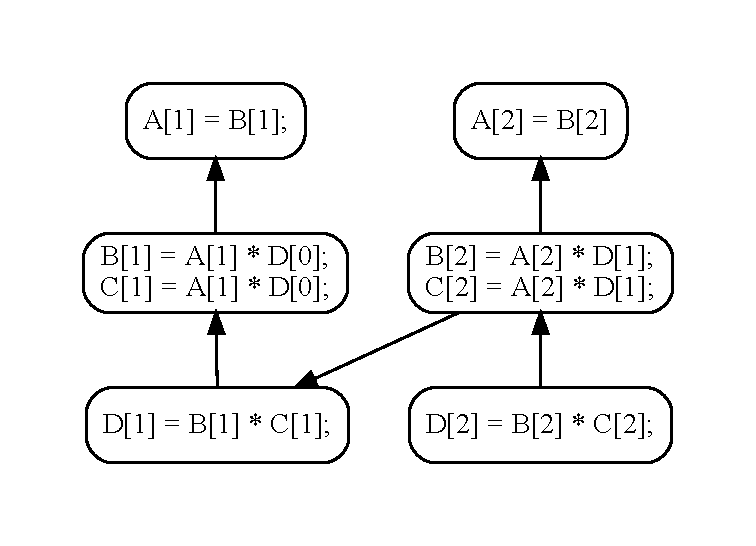
\includegraphics[width=\textwidth]{unrolledloopdep}
\end{minipage}
\caption{Dependencies for running example. %\figref{fig:flattenedloop}
%\lindsey{Ana, you can copy and paste this for the comment in
%\secref{sec:theoreticalguarentees}!}
}
\label{fig:unrolledloopdep}  
\end{figure}


\begin{figure}[h]
\centering
\begin{minipage}{\textwidth}
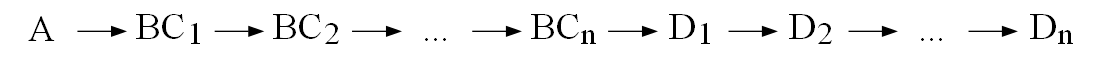
\includegraphics[width=\textwidth]{unrolledloopschedule}
\end{minipage}
\caption{Schedule for running example. %\figref{fig:flattenedloop} 
%\lindsey{Ana, you can copy and paste this for the comment in
%\secref{sec:theoreticalguarentees}!}
}
\label{fig:unrolledloopschedule}  
\end{figure}


We first consider the answer to Problem 1 (in MPC). 
We argue that optimal parallelization within a loop body is NP-complete (under the above stated assumptions). 
Therefore, compilers must resort to heuristics to compute a schedule for the instructions within a loop body.

We consider two operations, call them $A$ and $M$. Each instruction in the program is either an $A$-instruction or
an $M$-instruction. In order to benefit from parallelization/amortization, we must schedule two or more 
$A$-instructions in the same parallel node (or two or more $M$-instructions in the same parallel node). 
Scheduling $A$-instructions in parallel with $M$-instruction does not benefit from amortization.
It incurs the exact same cost as scheduling the $A$-instructions in a node $P_A$, scheduling the $M$-instructions 
in a node $P_M$, and having $P_A$ precede $P_M$ in the parallel schedule. This is the difference 
between classical scheduling, as studied in parallel computing, and MPC scheduling. 

We make the following assumptions:

\begin{enumerate}

\item $A$ and $M$ are of equal cost, 1 unit.
\item There is unlimited bandwidth---i.e., a single $A$-instrution (or $M$-instruction) costs as much as $N$ amortized $A$-instructions 
(or $M$-instructions), namely 1 unit.
 
\end{enumerate}

Consider a loop body that consists of $n$ sequences: $S_1$, ... $S_n$ of $A$ and $M$ instructions. 
More precisely, the loop body is such that its instructions can be grouped into such sequences. 
$S_1$, ... $S_n$ can execute in parallel, however, all instructions within a sequence must 
execute sequentially. For example, consider the three sequences (the right arrow indicates a \emph{dependence},
meaning that the source node must execute before the target node): 
\begin{enumerate}
\item $A \rightarrow M \rightarrow A$
\item $A \rightarrow A \rightarrow A$
\item $M \rightarrow A \rightarrow M$
\end{enumerate} 

A \emph{schedule} $P: P_1 \rightarrow P_2 \dots \rightarrow P_k$ is such that for each sequence 
$S_i$ in the set, if $S_i[k]$ precedes $S_i[k']$ in $S_i$ then $S_i[k]$ is scheduled in node $P_l$, $S_i[k]$ 
is scheduled in node $P_{l'}$, and $P_l$ precedes $P_{l'}$ in $P$. 

The cost of a schedule $P$ is 
\[\mathit{cost}(P) = \sum_{i=1}^k \mathit{cost}(P_i)\]
where $\mathit{cost}(P_i) = 1$ if $P_i$ consists of $A$-instructions only, or $M$-instructions only, 
and $\mathit{cost}(P_i) = 2$ if $P_i$ mixes $A$-instructions and $M$-instructions. 

The problem is to find a schedule $P$ with \emph{minimal cost}. For example, 
a schedule with minimal cost for the sequences above is
\[ A(1), A(2) \rightarrow M(1), A(2), M(3) \rightarrow A(1), A(2), A(3) \rightarrow M(3) \]
(The parentheses above indicate the sequence where the instruction comes from: (1), (2), or (3).)
The cost of this schedule is 5. 

The problem of finding a schedule with minimal cost 
easily reduces to the problem of finding a \emph{shortest common supersequence}, 
a known NP-complete problem \ana{citation needed}. To see the reduction, 
suppose $P$ is a schedule with minimal cost (computed by a black-box algorithm). 
We can derive a schedule $P'$ with the same cost as $P$, by mapping each mixed node $P_i \in P$ 
to two consecutive nodes in $P'$: an $A$-instruction node followed by an $M$-instruction node.
Clearly, $P'$, which now is a sequence of $A$'s and $M$'s, is a supersequence of each sequence 
$S_i$, i.e., $P'$ is a common supersequence 
of $S_1 \dots S_n$. It is also a shortest common supersequence. (To see this, suppose, a 
shorter common supersequence, $P''$, exists. $P''$ is a schedule of $S_1 \dots S_n$
and the $\mathit{cost}(P'')$ equals the length of $P''$. Since $P'$ is longer than
$P''$, and $\mathit{cost}(P') = \mathit{cost}(P)$, that means $\mathit{cost}(P'') < \mathit{cost}(P)$, 
which is a contradiction since $P$ is a schedule with minimal cost.)

\ana{Question: are these two assumptions too strong?} 

\ana{Assumption 1 can be relaxed --- e.g., if $A$ is 5 times cheaper than $M$, 
we can construct a program where all $A$'s are sequences of five consecutive 
$A$'s, which reduces to the previous problem.}

\ana{Assumption 2, I am not sure if this is acceptable, or maybe it is too strong. 
My intuition is that incorporating into the cost a dependence on the number 
of instructions in each parallel node, is going to make the problem harder, not easier...}

\section{Optimal Loop Parallelization} 
\label{sec:optimal_loop_parallelization}
%\input{../sections/optimal_loop_parallelization.tex}

\ana{Aiken's and Array SSA to define the notion of optimal loop parallelization for MPC.}

We now consider the answer to Problem 2 (in MPC). 

\subsection{Problem Overview} 

Recall Problem 2, given a loop-body schedule, compute the across-loop schedule
with minimal cost. The following examples illustrate. The first example is the inner 
product computation, and the second is Aiken and Nicolau's example.

\begin{tabular}{lll}
\begin{lstlisting}[language=Java]
A = ...
B = ...
ip = 0;
for (i=1; i<=N; i++) {
  t=A[i]*B[i];
  ip=ip+t;
}	

\end{lstlisting}
& 
~
&
\begin{lstlisting}[language=Java]
A = ...
B = ...
ip = 0;
for (i=1; i<=N; i++) {
  if (i%step5==1) para(t[i],...,t[i+step])
  if (i%step6==1) ip = ip + t[i];
}  
\end{lstlisting}

\end{tabular}

\ana{More to introduce what the schedule is.}

In the above example {\sf step5} is N, meaning that all N multiplications are executed in parallel.
In contrast, {\sf step6} is 1, meaning that the summation statements are executed sequentially.

A more interesting example involves array reads and writes. We return to the Aiken and Nicolau
example:

\begin{tabular}{lll}
\begin{lstlisting}[language=Java]
for (i=1; i<=N; i++) {
  A[i]=f1(B[i]);
  B[i]=f2(A[i],D[i-1]);
  C[i]=f3(A[i],D[i-1]);
  D[i]=f4(B[i],C[i]);
}	

\end{lstlisting}
& 
~
&
\begin{lstlisting}[language=Java]
for (i=1; i<=N; i++) {
  if (i%N==1) para(A[i]=f1(B[i]),...);
  if (i%1==1) para(B[i]=f2(A[i],D[i-1]),...);
  if (i%1==1) para(C[i]=f3(A[i],D[i-1]),...);
  if (i%1==1) para(D[i]=f4(B[i],C[i]),...);
}	
\end{lstlisting}

\end{tabular}

The above across-loop schedule means that the first instruction is parallelized---all
N instructions A can be computed at once because each depends only on {\sf B[i]}, which
is assigned outside of the loop. In contrast, subsequent instructions are executed 
sequentially. Take B, for example. There is a dependence ``cycle'' from {\sf B[i]} 
to {\sf D[i]} then {\sf B[i+1]} in the subsequent iteration. (The cycle is shown in~\figref{fig:MPCexample}(b).) 
{\sf B[i]}'s cannot be computed in parallel because each one depends on the {\sf B[i]} 
value computed in the previous iteration.

Now consider the above code but slightly modified. {\sf B[i]} and {\sf C[i]} are now 
computed based on the value of {\sf D[i]} from two iterations ago.

\begin{tabular}{lll}
\begin{lstlisting}[language=Java]
for (i=1; i<=N; i++) {
  A[i]=f1(B[i]);
  B[i]=f2(A[i],D[i-2]);
  C[i]=f3(A[i],D[i-2]);
  D[i]=f4(B[i],C[i]);
}	

\end{lstlisting}
& 
~
&
\begin{lstlisting}[language=Java]
for (i=1; i<=N; i++) {
  if (i%N==1) para(A[i]=f1(B[i]));
  if (i%2==1) para(B[i]=f2(A[i],D[i-2]));
  if (i%2==1) para(C[i]=f3(A[i],D[i-2]));
  if (i%2==1) para(D[i]=f4(B[i],C[i]));
}	
\end{lstlisting}

\end{tabular}

{\sf B[i]} still depends on values computed in earlier iterations, but one of the values, D[i-2] 
is two iterations earlier. Thus, we can take parallelization steps of 2, e.g., computing 
{\sf B[1]} and {\sf B[2]} in parallel, then {\sf B[3]} and {\sf B[4]} in parallel, etc.
Note however, that we cannot take a parallelization step larger than 2.
The value of B will depend on a value being computed in parallel.

To simplify, we assume that a loop-body schedule is a straight line. \ana{What does this mean?}
\ana{Will we relax?}
The problem therefore becomes: compute the maximal parallelization 
step allowed for each statement. This will account for an MPC schedule with
minimal cost. \ana{Why?}

\subsection{Preliminaries}

\ana{1. MPC-Source}

%\begin{figure*}[tbhp]
\begin{figure}[tbhp]
\begin{tabular}{ll}
\begin{minipage}[b]{4.25cm}

\begin{minted}[fontsize=\footnotesize, linenos, numbersep=5pt, escapeinside=||]{java}
// returns val%mod    
int rem(int val, int mod) {
  int rem = 0;
  for (int j = LEN-1; j |$\ge$| 0; j--) 
  {
    rem = rem << 1;
    // rem[0] = val[j]                                                                                                            
    rem = rem + ((val>>j)&1);   
    if (rem |$\ge$| mod) 
    {
      rem = rem - mod;
    }
  }    
  return rem;
}
\end{minted}
\end{minipage} 

&

\begin{minipage}[b]{4.25cm}
\begin{minted}[fontsize=\footnotesize, linenos, numbersep=5pt, escapeinside=||]{java}
// begin inlined rem
int rem0 = 0;
for (int j = LEN-1; j >= 0; j--) 
{
  rem1 = (j==LEN-1) ? rem0 : rem5;
  rem2 = rem1 << 1;
  rem3 = rem2 + (x1>>j)&1; 
  rem4 = rem3 - y1;
  cnd1 = CMP(rem3 >= y1);
  rem5 = MUX(rem3,rem4,cnd1);
}  
// end inline rem        
\end{minted}
\end{minipage}
\\

(a) Source 
&
(c) MPC-source

\end{tabular}
\caption{(a) shows standard (IMP-like) source for an MPC-friendly implementation 
of integer division~\cite{Demmler}, and (b) shows MPC-source. Line 5 {\sf rem1 = (j==LEN-1) ? rem0 : rem5;} 
is what we call a {\em pseudo-$\phi$} node. Note that the {\sf if}-statement on left
becomes straight-line code in MPC. The program \emph{runs both branches}, and 
at the end runs the conditional of the if-statement followed by the multiplexer. 
If {\sf cnd1} is {\sf true}, then {\sf rem} gets assigned the value along the left branch;
otherwise, it gets assigned the value along the right branch.}
    \label{fig:example}\vspace{-2ex}
\end{figure}


\paragraph{MPC-Source.} MPC-Source is an SSA-based intermediate representation
of MPC programs~\cite{ccs paper}. MPC-Source is, essentially, a straight-line sequence
of ``components'', where each ``component'' is either a nested for-loop sequence (called for-loop block), 
or a simple MPC-statement. \figref{fig:example} shows an example. MPC-Source can be constructed
in a standard way from an SSA-translation of the source---each branch of an 
{\sf if}-statement is added to the sequence, the conditional becomes an MPC comparison (CMP), 
and the $\phi$-node becomes an MPC multiplexer (MUX). 

\paragraph{Array SSA.} The other essential concept we build upon is Array SSA. Originally proposed 

\ana{3. MPC-Source with Array SSA}

\begin{lstlisting}[language=Java,escapeinside=`']
for (i=1; i<=N; i++) {

  Invariant: @A1[j] == j if `$j < i$', @A1[j] == 0 otherwise

  A1 = `$\phi$'(A3,A0); @A1 = max(A3,A0);  
  B1 = `$\phi$'(B3,B0); @B1 = max(B3,B0);
  C1 = `$\phi$'(C3,C0); @C1 = max(C3,C0);
  D1 = `$\phi$'(D3,D0); @D1 = max(D3,D0);

  A2[i] = f1(B1[i]); @A2[i] = i;
  A3 = `$\phi$'(A2,A1); @A3 = max(A2, A1);
  B2[i] = f2(A3[i],D1[i-1]); @B2[i] = i;
  B3 = `$\phi$'(B2,B1); @B3 = max(B2, B1);
  C3[i] = f3(A3[i],D1[i-1]); @C2[i] = i;
  C3 = `$\phi$'(C2,C1); @C3 = max(C2, C1);
  D3[i] = f4(B3[i],C3[i]); @D2[i] = i;
  D3 = `$\phi$'(D2,D1); @D3 = max(D2, D1); 
}
\end{lstlisting}

"Index invariant" makes an assertion about when A[i] is written as a function of i.
\ana{Figure out how to reason about cycles based on Array SSA.}

\subsection{Algorithm}

for a statement x = f(y,z), follow the reverse def-use link.

\section{Future Work}
\label{sec:implementation_and_benchmarks}
%\input{../sections/implementation_and_benchmarks.tex}
%\input{../sections/evaluation.tex}

\section{Conclusions}
\label{sec:conclusion}
%\input{../sections/conclusion.tex}

%\begin{acks}
%    \ishaq{TODO}
%\end{acks}

\printbibliography

% that's all folks
\end{document}


